\section{Observables}

\begin{frame}
	\frametitle{Observables}

	\begin{center}
	\alertb{\bf Classical Ising model}
	\begin{align}
		&M(t) = \frac{1}{L^2} \sum_{i} \braket{S_i}_t \,\,; \\
		&G(t,{\bm x},{\bm y}) \equiv \langle s_{\bm x}\, s_{\bm y}\,
		\rangle_t \,.
	\end{align}
	\end{center}
	\begin{center}
	\alertb{\bf Quantum models}\\
	Adiabaticity function:
	\begin{eqnarray}
  		A(t) = \Big|\braket{ \Psi_0[w(t)] | \Psi(t) }\Big|\,;
  		\label{adtfunc}
	\end{eqnarray}
	\end{center}
	
	%\begin{columns}
	%\begin{column}{0.5\textwidth}
	%\begin{center}
	%{\bf Ising:}
	%\begin{align}
	%	M(t) \equiv {1\over L} \sum_x  \langle \Psi(t) | \, \sigma_x^{(1)}
	%	| \Psi(t) \rangle\,;
	%	\notag
	%\end{align}
	%\end{center}
	%\end{column}
	%\begin{column}{0.4\textwidth}
	\begin{center}
	{\bf Kitaev:}
	\begin{align}
		C(x,t)  \equiv  \langle \Psi(t) |
  		\, c_j^\dagger c_{j+x} 
  		+ c_{j+x}^\dagger c_{j} \, | \Psi(t) \rangle \, \, . \notag
	\end{align}
	\end{center}
	%\end{column}
	%\end{columns}
	
	
\end{frame}


\begin{frame}
	\frametitle{The Round-Trip}

	\begin{center}
		\begin{figure}
					   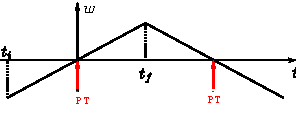
\includegraphics[width=10.4cm]{paper/protocol.pdf}
					  \caption{ Round-trip Protocol: the intersection with the x-axis corresponds to the phase transition (PT) point.  }
					\label{protocol}
		\end{figure}
	\end{center}
	
	
	
\end{frame}